\documentclass[%
	11pt,
	a4paper,
	utf8,
	%twocolumn
		]{article}	

\usepackage{style_packages/podvoyskiy_article_extended}


\begin{document}
\title{Общие и специальные вопросы оптимизации}

\author{\itshape Подвойский А.О.}

\date{}
\maketitle

\thispagestyle{fancy}

%Здесь приводятся заметки по специальным вопросам теории оптимизации


%\shorttableofcontents{Краткое содержание}{1}

\tableofcontents

\section{Полезные ссылки}

\url{https://mujoco.org/}

Элегантный фреймворк для RL (NB!): \url{https://github.com/thu-ml/tianshou}

Фреймворк JORDLY: \url{https://github.com/kakaoenterprise/JORLDY}

Курс по прикладному RL: \url{https://github.com/yandexdataschool/Practical_RL}

Курс Сергея Левина: \url{https://www.youtube.com/playlist?list=PL_iWQOsE6TfURIIhCrlt-wj9ByIVpbfGc}

\section{Задача обучения с подкреплением}

Под желаемым результатом мы будем понимать максимизацию некоторой скалярной величины, называемой \emph{наградой} (reward). Интеллектуальную сущность (систему/робота/алгоритм), принимающую решения, будем называть \emph{агентом} (agent).

Агент взаимодействует с миром или \emph{средой} (environment), которая задается зависящем от времени \emph{состоянием} (state). Агенту в каждый момент времени в общем случае доступно только некоторое \emph{наблюдение} (observation) текущего состояния мира. Сам агент задает процедуру выбора \emph{действия} (action) по доступным наблюдениям; эту процедуру далее будем называть \emph{стратегией} или \emph{политикой} (policy). Процесс взаимодействия агента и среды задается \emph{динамикой среды} (world dynamics), определяющей правила смены состояний среды во времени и генерации награды.

Буквы $ s $, $ a $, $ r $ зарезервируем для состояний, действий и наград соответственно. Буквой $ t $ будем обозначать время в процессе взаимодействия.

\subsection{Модель взаимодействия агента со средой}

\subsubsection{Марковская цепь}

\emph{Свойство Марковости}: процесс зависит только от текущего состояния и не зависит от всей предыдущей истории. 

\emph{Марковской цепью} (Markov chain) называется пара $ (\mathcal{S}, \mathcal{P}) $, где $ \mathcal{S} $ -- множество состояний, а $ \mathcal{P} $ -- вероятности переходов $ \{ p(s_{t+1} | s_t) | t \in \{0, 1, \ldots, \}, s_t, s_{t+1} \in \mathcal{S} \} $.

Марковская цепь называется \emph{однородной} или \emph{стационарной}, если вероятности переходов не зависят от времени
\begin{align*}
	\forall t: p(s_{t+1} | s_t) = p(s_1 | s_0).
\end{align*}

По определению, переходы $ \mathcal{P} $ стационарных марковских цепей задаются единственным условным распределением $ p(s' | s) $. Апостроф канонично используется для обозначения <<следующих>> моментов времени.

\subsubsection{Среда / Окружение}

\emph{Средой} (environment) называется тройка $ \mathcal{S}, \mathcal{A}, \mathcal{P} $, где $ \mathcal{S} $ -- множество (пространство) состояний, $ \mathcal{A} $ -- множество (пространство) действий, $ \mathcal{P} $ -- функция переходов или динамика среды: вероятности $ p(s' | s, a) $.

\remark{%
Если среда не является полностью наблюдаемой, задача существенно усложняется, и необходимо переходить к формализму частично наблюдаемых MDP (partially observable MDP, PoMDP)
}

\subsubsection{Действия}

Нас будут интересовать два вида пространства действий $ \mathcal{A} $:
\begin{itemize}
	\item конечное, или \emph{дискретное пространство действий} (discrete action space): $ | \mathcal{A} | < + \infty $. Мы также будем предполагать, что число действий $ | \mathcal{A} | $ достаточно мало,
	
	\item \emph{непрерывное пространство действий} (continuous domain): $ \mathcal{A} \subseteq [-1, 1]^m $. Выбор именно отрезков $ [-1, 1] $ не является ограничивающем общности распространенным соглашением. Задачи с таким пространством действий также называют задачами непрерывного управления.
\end{itemize}

\subsubsection{Траектории}

Набор $ \mathcal{T} := (s_0, a_0, s_1, a_1, s_2, a_2, \ldots) $ называется \emph{траекторией}.

Для данной среды, политики $ \pi $ и начального состояния $ s_0 \in \mathcal{S} $ распределение, из которого приходят траектории $ \mathcal{T} $, называется \emph{trajectory distibution}
\begin{align*}
	p(\mathcal{T}) = p(a_0, s_1, a_1, \ldots) = \prod_{t \geqslant 0} \pi (a_t | s_t) \, p(s_{t+1} | s_t, a_t)
\end{align*}

Мы часто будем рассматривать \emph{мат. ожидание по траекториям}, которые будем обозначать $ \mathbb{E}_{\mathcal{T}} $. Под этим подразумевается бесконечная цепочка вложенных мат. ожиданий
\begin{align*}
	\mathbb{E}_{\mathcal{T}} = \mathbb{E}_{\pi (a_0 | s_0)} \mathbb{E}_{p(s_1 | s_0, a_0)} \mathbb{E}_{\pi(a_1 | s_1)} \cdots (\cdot)
\end{align*}

Поскольку часто придется раскладывать эту цепочку, договоримся о следующем сокращении
\begin{align*}
	\mathbb{E}_{\mathcal{T}} (\cdot) = \mathbb{E}_{a_0} \mathbb{E}_{s_1} \mathbb{E}_{a_1} \ldots (\cdot)
\end{align*}

Однако в такой записи стоит помнить, что действия приходят из некоторой зафиксированной политики $ \pi $, которая неявно присутствует в выражении. Для напоминания об этом будет, где уместно, использоваться запись $ \mathbb{E}_{\mathcal{T} \sim \pi} $.

\subsubsection{Марковский процесс принятия решений (MDP)}

Для того, чтобы сформулировать задачу, нам необходимо в среде задать агенту цель -- некоторый функционал для оптимизации. По сути, марковский процесс принятия решений -- это среда плюс награда.

Мы будем пользоваться следующим определением: \emph{Марковский процесс принятия решений} (Markov Decision Process, MDP) -- это четверка $ (\mathcal{S}, \mathcal{A}, \mathcal{P}, r) $, где
\begin{itemize}
	\item $ \mathcal{S}, \mathcal{A}, \mathcal{P} $ -- среда,
	
	\item $ r: \mathcal{S} \times \mathcal{A} \rightarrow \mathbb{R} $ -- \emph{функция вознаграждения} (reward function).
\end{itemize}

Сам процесс выглядит следующим образом. Для момента времени $ t = 0 $ начальное состояние мира полагается $ s_0 $. Агент наблюдает все состояние целиком и выбирает действие $ a_0 \in \mathcal{A} $. Среда отвечает генерацией награды $ r(s_0, a_0) $ и сэмплирует следующее состояние $ s_1 \sim p(s' | s_0, a_0) $. Агент выбирает $ a_1 \in \mathcal{A} $, получает вознаграждение $ r(s_1, a_1) $, состояние $ s_2 $, и так далее до бесконечности.

\remark{
Считать функцию вознаграждения \emph{детерминированной} удобно, поскольку позволяет не городить по ним мат. ожидания (иначе нужно добавлять сэмплы наград в определение траектории)
}

В любом формализме всегда принято считать, что агент сначала получает награду и только затем наблюдает очередное состояние.

Марковский процесс принятия решений (MDP) называется \emph{конечным} (finite MDP) или табличным, если пространства состояний и действий конечны: $ |\mathcal{S}| < \infty $, $ | \mathcal{A} < \infty | $.

\subsubsection{Эпизодичность}

Во многих случаях процесс взаимодействия агента со средой может при определенных условиях <<заканчиваться>>, причем факт завершения доступен агенту.

Состояние $ s $ называется \emph{терминальным} (terminal) в MDP, если $ \forall a \in \mathcal{A} $:
\begin{align*}
	\mathbb{P}(s' = s | s, a) = 1, \quad r(s, a) = 0,
\end{align*}
то есть с вероятностью 1 \underline{агент не сможет покинуть состояние}.

Считается, что на каждом шаге взаимодействия агент дополнительно получает для очередного состояния $ s $ значение предиката $ done(s) \in \{0, 1\} $, является ли данное состояние терминальным. По сути, после попадания в терминальное состояние дальнейшее взаимодействие бессмысленно (дальнейшие события тривиальны), и, считается, что возможно произвести $ reset $ среды в $ s_0 $, то есть начать процесс взаимодействия заново.

Один цикл процесса от стартового состояния до терминального называется \emph{эпизодом} (episode). Продолжительности эпизодов (количество шагов взаимодействия) при этом, конечно, могут различаться от эпизода к эпизоду.

Среда называется \emph{эпизодичной} (episodic), если для любой стратегии процесс взаимодействия гарантированно завершается не более чем за некоторое конечное $ T^{\max} $ число шагов.

\remark{
В эпизодичных средах вероятность оказаться в одном и том же состоянии дважды равна нулю
}

На практике, в средах обычно существуют терминальные состояния, но нет гарантии завершения эпизодов за ограниченное число шагов. Это лечат при помощи таймера -- жесткого ограничения, требующего по истечении $ T^{\max} $ шагов проводить в среде ресет.

\subsubsection{Дисконтирование}

Наша задача заключается в том, чтобы найти стратегию $ \pi $, максимизирующую среднеюю суммарную награду. Формально, нам явно задан функционал для оптимизации
\begin{align*}
	\mathbb{E}_{\mathcal{T} \sim \pi} \sum_{t \geqslant 0} r_t \rightarrow \underset{\pi}{\max},
\end{align*}
где $ r_t := r(s_t, a_t) $ -- награда на шаге $ t $.

Мы хотим исключить из рассмотрения MDP, где данный функционал может улететь в бесконечность или не существовать вообще. Во-первых, введем ограничение на модуль награды за шаг, подразумевая, что среда не может поощрять или наказывать агента бесконечно сильно
\begin{align}\label{eq:rl-discont}
	\forall s, a: | r(s, a) | \leqslant r^{\max}
\end{align}

Чтобы избежать парадоксов, этого условия нам не хватит. Введем \emph{дисконтирование} (discounting), коэффициент которого традиционно обозначают $ \gamma $.

\emph{Дисконтированной кумулятивной наградой} (discounted cumulative reward) или \texttt{total return} для траектории $ \mathcal{T} $ с коэффициентом $ \gamma \in (0, 1] $ называется
\begin{align*}
	R(\mathcal{T}) := \sum_{t \geqslant 0} \gamma^t r_t
\end{align*}

У дисконтирования есть важная интерпретация \cite[\strbook{13}]{ivanov:rl-2022}: мы полагаем, что на каждом шаге с вероятностью $ 1 - \gamma $ взаимодействие обрывается, и итоговым результатом агента является та награда, которую он успел собрать \underline{до прерывания}. Это дает приоритет получению награды в \emph{ближайшее} время перед получением той же награды через некоторое время. Математически смысл дисконтирования в том, чтобы в совокупности с требованием \eqref{eq:rl-discont} гарантировать ограниченность оптимизируемого функционала.

\emph{Скором} (score  или performance) стратегии $ \pi $ в данном MDP называется \cite[\strbook{13}]{ivanov:rl-2022} 
\begin{align*}
	J(\pi) := \mathbb{E}_{\mathcal{T} \sim \pi} R(\mathcal{T})
\end{align*}

Итак, задачей обучения с подкреплением является оптимизация для заданного MDP средней дисконтированной кумулятивной награды
\begin{align*}
	J(\pi) \rightarrow \underset{\pi}{\max}
\end{align*}

То есть, другими словами, мы ищем наиболее эффективную стратегию $ \pi $, которая максимизирует среднее накопленное вознаграждение.

\subsection{Алгоритмы обучения с подкреплением}

Классификация наиболее популярных алгоритмов приведена на 

\begin{figure}[h]
	\centering
	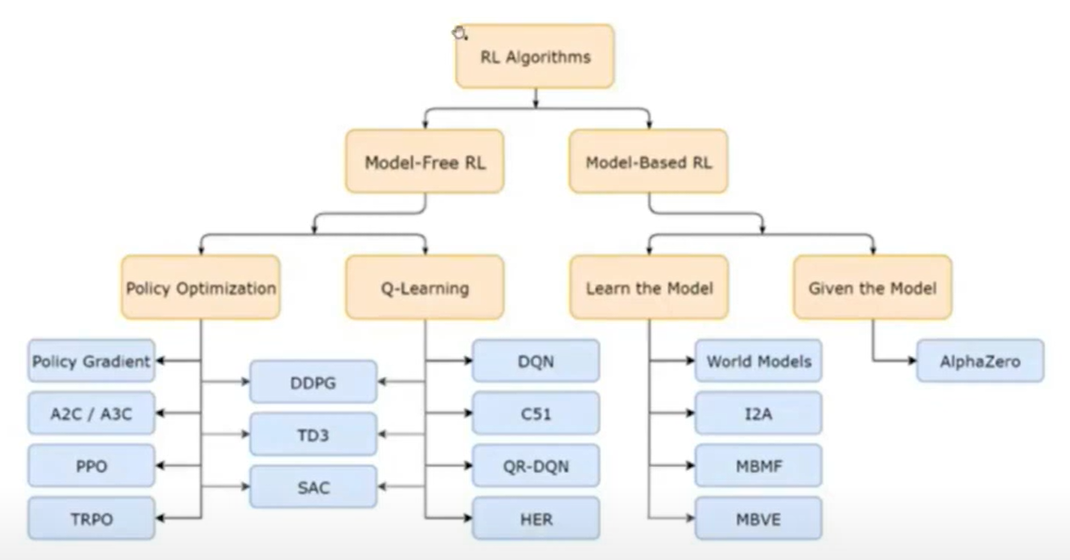
\includegraphics[scale=0.85]{figures/classif_rl_algo.png}
	\caption{ Классификация алгоритмов обучения с подкреплением }\label{fig:classif_rl_algo}
\end{figure}

\subsubsection{Условия задачи RL}

Основной постановкой в обучении с подкреплением является задача нахождения оптимальной стратегии на основе собственного опыта взаимодействия. Это означает, что алгоритму обучения изначально доступно только:
\begin{itemize}
	\item вид пространства состояний -- количество состояний в нем в случае конечного числа, или размерность пространства $ \mathbb{R}^d $ в случае признакового описания состояний,
	
	\item вид пространства действий -- непрерывное или дискретное. Некоторые алгоритмы будут принципиально способны работать только с одним из этих двух видов,
	
	\item взаимодействие со средой, то есть возможность для предоставленой алгоритмом стратегии $ \pi $ генерировать траектории $ \mathcal{T} \sim \pi $; иными словами, принципиально доступны только сэмплы из trajectory distribution.
\end{itemize}

Итак, в отличие от обучения с учителем, где датасет <<дан алгоритму на вход>>, здесь агент должен сам собрать данные. Находясь в некотором состоянии, обучающийся агент обязан выбрать ровно одно действие, получить ровно один сэмпл $ s' $ и продолжить взаимодействие (накопление опыта -- сбор сэмплов) из $ s' $. Собираемые в ходе взаимодействия данные и представляют собой всю доступную агенту информацию для улучшения стратегии.

Пятерки $ \mathbb{T} := (s, a, r, s', done) $, где $ r := r(s, a) $, $ s' \sim p(s' | s, a) $, $ done := done(s') $.

Таким образом, в RL-алгоритме должна быть прописана стратегия взаимодействия со средой во время обучения (behavior policy), которая может отличаться от <<итоговой>> стратегии (target policy), предназначенной для использования в среде по итогам обучения.

Необходимость собирать данные внутри самого алгоритма -- одно из ключевых отличий задачи RL от обучения с учитилем, где выборка подается алгоритму на вход.

Доступной помощью для алгоритма могут быть данные от эксперта, то есть записи взаимодействия со средой некоторой стратегии (или разных стратегий), не обязательно, вообще говоря, оптимальной. Алгоритмы RL, возможно, сможет эти данные как-то использовать, или хотя бы как-либо на них предобучиться.

В простейшем случае предобучение выглядит так: если в алгоритме присутствует параметрически заданная стратегия $ \pi_{\theta} $, можно \emph{клонировать поведение} (behavior cloning), т.е. восстанавливать по парам $ s, a $ из всех собранных экспертом траекторий функцию $ \mathcal{S} \rightarrow \mathcal{A} $ (это обычная задача обучения с учителем), учиться воспроизводить действия эксперта.

Задача обучения по примерам ее решения около-оптимальным экспертом называется \emph{имитационным обучением} (imitation learning). Однако, если эксперт не оптимален, обученная стратегия вряд ли будет действовать хоть сколько-то лучше. Здесь можно провести прямую аналогию с задачей обучения с учителем, где верхняя граница качества алгоритма определяется качеством разметки; если разметка зашумлена и содержит ошибки, обучение вряд ли удастся.

\subsubsection{Концепция model-free алгоритмов}

Алгоритм RL классифицируется как \emph{model-free}, если он не испольузет и не пытается выучить модель динамики среды $ p(s' | s, a) $.

\subsubsection{On-policy vs Off-policy}

Алгоритм RL называется \emph{off-policy}, если он может использовать для обучения опыт взамодействия произвольной стратегии.

Алгоритм RL называется \emph{on-policy}, если для очередной итерации алгоритма ему требуется опыт взаимодействия некоторой конкретной, предоставляемой самим алгоритмом, стратегии.

Off-policy алгоритм должен уметь проводить очередной шаг обучения на произвольных траекториях, сгенерированных произвольными (возможно, разными, возможно, неоптимальными) стратегиями. Понятие принципиально важно тем, что алгоритм может потенциально переиспользовать траектории, полученные старой версией стратегии со сколь угодно давних итерации.

Если алгоритм может переиспользовать опыт, но с ограничениями (например, только с недавних итераций, или только из наилучших траекторий), то мы все равно будем относить его к on-policy, поскольку для каждой новой итерации алгоритма нужно будет снова собирать сколько-то данных. 

Важно, что off-policy алгоритм сможет на данных произвольного эксперта провести <<полное>> обучение, то есть условно сойтись к оптимуму при достаточном объеме и разнообразии экспертной информации, не потребовав вообще никакого дополнительного взаимодействия со средой.

\subsubsection{Классификация RL-алгоритмов}

Model-free алгоритмы часто делят на следующие подходы:
\begin{itemize}
	\item мета-эвристики,
	
	\item value-based,
	
	\item policy gradient.
\end{itemize}

\subsubsection{Сложности задачи RL}

\emph{Проблема застревания в локальных оптимумах} приходит напрямую из методов оптимизации. Другие проблемы куда более характерны именно для RL. Допустим, агент совершает какое-то действие, которое запускает в среде некоторый процесс. Процесс протекает сам по себе без какого-либо дальнейшего вмешательства агента и завершается через много шагов, приводя к награде. Это \emph{прблема отложенного сигнала} (delayed reward) -- среда дает фидбэк агенту спустя какое-то (вообще говоря, неограниченно длительное) время.

Поскольку функция награды может быть произвольная, довольно типично, когда сигнал от среды -- неконстантная награда за шаг -- приходит очень редко. Это проблема \emph{разреженной награды} (sparse reward).

Еще одна очень важная проблема -- \emph{дилемма исследования-использования} (exploration-exploitation trade-off). 

\subsubsection{Дизайн функции награды}

И есть еще одна, вероятно, главная проблема. Откуда берется награда? Алгоритмы RL предполагают, что награда, как и среда, заданы, <<поданы на вход>>, и эту проблему наши алгоритмы обучения, в отличие от предыдущих, решать идеологически не должны.

Но понятно, что если для практического применения обучения с учителем боттлнеком часто является необходимость размечать данные -- <<предоставлять обучающий сигнал>> -- то в RL необходимо аккуратно описать задачу при помощи функции награды.

Общее практическое правило звучит так: хорошая функция награды поощряет агента за достигнутые результаты, а не за то, каким способом агент этих результатов добивается. Это логично: если вдруг дизайнеру награды кажется, что он знает, как решить задачу, то вероятно, RL не особо и нужен. К сожалению, такая <<хорошая>> функция награды обычно разреженная.

Пусть дана некоторая функция $ \Phi (s): \mathcal{S} \rightarrow \mathbb{R} $, которую назавем \emph{потенциалом}, и которая удовлетворяет двум требованиям: она ограничена и равна нулю в терминальных состояниях. Будем говорить, что мы проводим reward shaping при помощи потенциала $ \Phi(s) $, если мы заменяем функцию награды по следующей формуле
\begin{align}\label{eq:reward_shaping}
	r^{new}(s, a, s') := r(s,a) + \gamma \Phi (s') - \Phi(s)
\end{align}

На практике reward shaping -- это инструмент внесения каких-то априорных знаний. Проведение любого reward shaping по формуле \eqref{eq:reward_shaping} не меняет задачи.




\listoffigures\addcontentsline{toc}{section}{Список иллюстраций}

% Источники в "Газовой промышленности" нумеруются по мере упоминания 
\begin{thebibliography}{99}\addcontentsline{toc}{section}{Список литературы}
	\bibitem{ivanov:rl-2022}{\emph{Иванов} Конспект по обучению с подкреплением, 2022}
	
	\bibitem{panteleev}{\emph{Пантлеев А. В., Летова Т.А,} Методы оптимизации в примерах и задачах. -- СПб.: Издательство <<Лань>>, 2015. -- 512 с.}
	
	\bibitem{vorontsova:convex_opt-2021}{\emph{Вороноцова Е.А.} Выпуклая оптимизация. -- М.: МФТИ, 2021. -- 364 с.}
	
	\bibitem{burkov:2020}{\emph{Бурков А.} Машинное обучение без лишних слов. -- СПб.: Питер, 2020. -- 192 с.}
		
	\bibitem{beazley:python-2010}{\emph{Бизли Д.} Python. Подробный справочник. -- Пер. с англ. -- СПб.: Символ-Плюс, 2010. -- 864~с. }
\end{thebibliography}

\end{document}
